\documentclass[a4paper,twocolumn,10pt,openany,oneside,final,fleqn]{memoir}

\usepackage{siunitx}
\usepackage[margin=2.5cm]{geometry}
\usepackage{libertine}
\usepackage{inconsolata}
\usepackage{graphicx}
\usepackage{booktabs}
%\usepackage{multicol}
\usepackage{float}
\usepackage{hyperref}
\usepackage[nameinlink]{cleveref}
\usepackage{xcolor}
\usepackage{cancel}
\usepackage{ccicons}
\usepackage{todonotes}
\usepackage{nicefrac}

\hypersetup{
    colorlinks,
    linkcolor={red!50!black},
    citecolor={blue!50!black},
    urlcolor={blue!80!black}
}

\nonzeroparskip
\raggedbottom

\setcounter{tocdepth}{2}


\newcommand{\Pos}[1]{{\ensuremath{+}#1}}
\newcommand{\Neg}[1]{{\ensuremath{-}#1}}
\newcommand{\Model}{MOD12003\ }
\newcommand{\rd}[1]{\texttt{#1}}
\newcommand{\xcircuit}[1]{ \centering \textsf{ \input{#1} } }

\setlength{\parskip}{3mm}

\title{\Model reference manual}
\author{NIHLabs}

\begin{document}

\frontmatter

\onecolumn
\begin{titlingpage}
\begin{tabularx}{\textwidth}{Xr}
\hline
\\
{\LARGE OWNER'S AND SERVICE MANUAL} &
\Model \\
\\
\hline
\end{tabularx}
\vfill
\begin{center}
    The \Model is a standard-precision, \SI{20}{V}, \SI{3}{A} module for the
    MOD1 series of multi-output, modular power supplies. It uses a hybrid
    switching + linear architecture that achieves acceptable noise levels for
    most uses while also maintaining low power dissipation.
\end{center}
\vfill
\begin{table}[h]
\centering
\caption{Specifications}
\begin{tabular}{p{2mm}lcc}
    \toprule
    \multicolumn{2}{l}{\textbf{Parameter}} & \textbf{Value} & \textbf{Unit} \\ \midrule
    \multicolumn{2}{l}{\textbf{Voltage}} & & \\ \midrule
    & Full-scale output voltage & 20 & V \\
    & Output voltage resolution & 10 & mV \\
    & Output voltage tolerance  & 0.5\% $\pm$ 10 & mV \\
    & Minimum output-enabled voltage & 100 & mV \\
    \midrule
    \multicolumn{2}{l}{\textbf{Current}} & & \\ \midrule
    & Full-scale output current & 3 & A  \\
    & Output current resolution & 2 & mA \\
    & Output current tolerance  & 0.5\% $\pm$ 2 & mA \\
    & Min. current limit, worst case & 10 & mA \\
    & Current sense dead zone, worst case   & 0 -- 10 & mA \\
    \midrule
    \multicolumn{2}{l}{\textbf{Slew rate} (software programmable)} & & \\ \midrule
    & Max. rising slew rate (allow 2\% + \SI{15}{mV} overshoot) & 3.2 & V/ms \\
    & Max. rising slew rate (no overshoot) & 2.0 & V/ms \\
    & Falling slew time constant (first-order RC) & 200 & ms \\
    \midrule
    \multicolumn{2}{l}{\textbf{Overload}} & & \\ \midrule
    & Max. forced pos. output voltage (passive) & 24 & V \\
    & Max. forced pos. output voltage (fuse blows) & 63 & V \\
    & Max. forced neg. output voltage (passive) & \Neg{0.3} & V \\
    & Max. forced neg. output voltage (fuse blows) & \Neg{63} & V \\
    & Fuse rupture capacity & 50 & A \\
    & On-board spare fuses (install with solder bridge) & 2 & \\
    & Programmable OVP (blows fuse if necessary) & 3 -- 24 & V \\
    & OVP threshold resolution & 150 & mV \\
    & OVP threshold tolerance  & 2\% $\pm$ 50 & mV \\
    \bottomrule
\end{tabular}
\end{table}
\vfill
\begin{center}
    \ccZero. No copyright claimed;
    \href{https://creativecommons.org/publicdomain/zero/1.0/}{Creative Commons Zero} where not possible.
    Written in 2015 by Chris Pavlina.
\end{center}
\end{titlingpage}

\clearpage
\twocolumn[
    \tableofcontents
]
\twocolumn[
    \listoffigures*
    \listoftables*
]

\mainmatter

\chapter{Theory of Operation}

\section{Introduction}

This chapter describes the operation of the \Model, ranging from a broad overview
to detailed sections on subcircuits and software routines.

\subsection{Block Diagram}

\begin{figure*}
\xcircuit{BlockDiagram}
\caption{Block diagram}\label{fig:blockdiagram}
\end{figure*}

\Cref{fig:blockdiagram} contains a block diagram of the \Model.

The \Model uses a standard, high-side regulation architecture. A \SI{24}{V} input
passes through an input protection block (including reverse polarity blocking and
inrush current limiting / bulk capacitance isolation) and directly into a software-controlled
buck converter. The output of this converter then passes through a linear regulator
stage and to the output. The output voltage is sensed directly at the output connector
and passes back to both the linear regulator and the microcontroller.

The output is fused, protecting internal circuitry in the event that power
is applied to the outputs externally, and helping to minimize damage to both the
\Model and to the device to which power is being supplied if the \Model fails.

The standard MOD1 serial loop interface feeds a capacitive coupler and is
processed directly by the microcontroller; passthrough to downstream modules is
also handled in software.

\section{Detailed Description}

\subsection{Microcontroller}

The Microcontroller is the device in control of the entire system. It receives signals
from the MOD1 motherboard, storing the desired output voltage, current, and slew rate.
These, combined with stored calibration data, are used to choose setpoints for both the
Preregulator and the Linear Regulator. Status signals from these circuits, including
the output voltage and current, regulation mode, and heat sink temperature, are monitored.
These all provide feedback for multiple safety and limiting functions.

\subsubsection{Calibration}

There are two major sources of error that must be corrected; calibration accounts for the
first one. This is manufacturing tolerance in the voltage sense and current sense amplifiers
and in the system voltage reference, which could cause the supply to read its own outputs
incorrectly and deliver an erroneous level.

To perform adjustment, the Microcontroller configures the regulators for four test points:
approximately 10\% and 90\% of full scale for both current and voltage. These initial
setpoints need not be correct. After they have stabilized, both the Microcontroller and
a human operator individually measure the actually achieved value, and the operator-supplied
measurement is entered into the system. These points are used to apply a linear correction
to the data read by the Analog-Digital Converter.

\subsubsection{Voltage Control Loop}

The second major source of error is inaccuracy and drift in the Linear Regulator.
The error amplifiers in this are not required to be accurate initially or in the long
term. As such, they may have significant offset voltage, and this offset voltage may
change significantly over temperature variants and time.

This error is removed by a self-correcting control loop implemented in the Microcontroller.
The Analog-Digital Converter digitizes the signals from the Sense Amplifiers, and calibration
is applied. The corrected value of the output voltage is compared to the desired output
voltage, and this error serves as the input to a control loop that corrects the error.

Because this error source is slow, this control loop is designed to be slow and gentle
to avoid loop stability interactions between it and the tighter, faster loops of the
Linear Regulator.

The use of such a correcting loop is a decision that was made to reduce complexity
and expense in the hardware of the Linear Regulator. Because the required connections
and peripherals in the Microcontroller were already in use, the Voltage Control Loop could
be added at the cost of only a few lines of firmware code, allowing the error amplifier
in the Linear Regulator to consist of only two very modest operational amplifiers.

\subsubsection{Overvoltage Protection}

The \Model's overvoltage protection is a system involving two
control methods. At its heart is a thyristor connected across the supply outputs.
Current supplied to the thyristor's gate bias circuit will cause it to
latch closed-circuit, conducting current until the output fuse opens.

A comparator is constantly comparing the output voltage, as read by the Sense Amplifier,
to a reference signal. This reference signal is supplied by the Microcontroller as a
pulse width modulated (PWM) waveform and filtered to produce a fixed level. If at any moment
the output voltage exceeds this point, the comparator alternates, saturating a transistor
that drives the thyristor's gate into conduction.

Due to the inaccurate nature of the PWM-derived level, this analog method is only used
for fast reponse and as a last resort if the Microcontroller stops functioning
\footnote{The PWM signal is generated by a relatively isolated peripheral inside the
    Microcontroller, which is expected to continue operation in the event of software
    errors or freezes.}.
More accurate protection is provided by the Microcontroller firmware. If the output
voltage is detected beyond a narrow margin above the setpoint, the PWM signal will
saturate, quickly forcing the thyristor into conduction regardless of the output
voltage as seen by the comparator.

\subsubsection{Group Error Response}

In an environment where multiple supply modules are used to power multiple rails of a
single device, it may be desirable to have so-called Group Error Response. The
Microcontroller detects multiple error conditions, including overvoltage protection trip,
output current exceeding a set value (if desired, with a fixed grace period to allow
inrush currents), thermal overload, and oscillation of the Linear
Regulator. If Group Error Response is configured, the selected error conditions will
cause the Microcontroller to notify all the other modules in the MOD1 system, prompting
the entire system to shut down as a precaution.

\subsection{Preregulator}

To allow substantial amounts of power to be delivered by a relatively small supply module,
a relatively high-efficiency buck-mode DC-DC converter is employed. This is controlled by
a pulse-width modulated waveform from the Microcontroller. An amplifier translates and shifts
the signal to provide a \SI{0}{V} to \SI{-14}{V} (relative to the positive supply) gate
drive waveform to a power P-channel MOSFET. The MOSFET, in conjunction with a Schottky
diode, chops the supply into a square wave which is then filtered by an LC filter circuit.

Software control allows the Preregulator to be controlled in a way that is most suitable
for a hybrid power supply. Under higher power conditions, the voltage drop across the Linear
Regulator will be minimized to keep its temperature low. Only a small amount of voltage
`headroom' is required to maintain an acceptable transient response. However, this is not
optimal under lower power conditions. The regulator would switch into `discontinuous' mode,
meaning that the MOSFET and diode are not always conducting. There is a dead time during
which output current is supplied only by the filter capacitors. This increases output voltage
ripple and high-frequency noise (the latter due to the ringing that is usually present in
the system when the normally driven `switching node' becomes a high impedance). When the
output power level is low enough for this to happen, it will also be low enough for the
Linear Regulator to provide all regulation by itself, and so the Microcontroller will
simply switch the MOSFET `on' and allow the full input voltage to reach the Linear Regulator.

\subsection{Linear Regulator}

Despite the efficiency benefit of the buck converter, it is not ideal. A switching converter's
output has a large amount of voltage ripple and it does not have a particularly nice transient
response. To convert the output of the Preregulator into a sufficiently clean supply, a Linear
Regulator passes and regulates the supply.

\subsubsection{Control Amplifiers}

\begin{figure}
\xcircuit{control358}
\caption{Linear regulator partial: control amplifier}
\label{fig:controlamp}
\end{figure}

\Cref{fig:controlamp} shows a simplified, partial schematic of the control amplifier.
Operational amplifier \rd{U2B} compares the voltage setpoint to the voltage feedback,
driving the output amplifier through switching diode pair \rd{D3}. Likewise, operational
amplifier \rd{U2A} compares the current setpoint to the current feedback, also driving
the output amplifier through \rd{D3}. The switching diode pair ensures that the output
amplifier is driven by whichever of the two control amplifiers is producing the smaller
signal, allowing either amplifier to `limit' the other.

\subsubsection{Output Amplifier}

\begin{figure}
\xcircuit{outamp}
\caption{Linear regulator partial: output amplifier}
\label{fig:outputamp}
\end{figure}

\Cref{fig:outputamp} shows a simplified schematic of the output amplifier. \rd{Q10}
and \rd{Q12} form a complementary feedback pair to supply the output current, and
two ferrite beads stabilize the pair against layout-induced oscillation. \rd{Q11}
buffers the output signal further to ensure that even when manufacturing variations
give low current gain in the \rd{Q10}, a relatively high resistor can supply the
bias to the output amplifier.

Diode pair \rd{D4} protects the emitter-base junctions of \rd{Q11} and \rd{Q12} in
the case that the output voltage is externally forced above the setpoint.

\subsection{Sense Amplifiers}

\begin{figure}
\xcircuit{vsense}
\caption{Voltage sense amplifier}
\label{fig:vsense}
\end{figure}

\begin{figure}
\centering
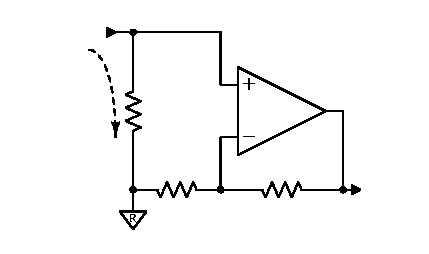
\includegraphics{isense}
\caption{Current sense amplifier}
\label{fig:isense}
\end{figure}

\Cref{fig:vsense} shows a simplified schematic of the voltage sense amplifier. This
is a differential amplifier that translates the output voltage, as detected between
the positive and negative output connectors, onto the system's internal \SI{0}{V}
reference potential. This is multiplied by the gain, which in this case is below
unity: $\nicefrac{1}{11}$. A sub-unity gain allows the relatively large output voltage
to be scaled into a range that is acceptable to the Microcontroller's analog-digital
and digital-analog converters.

\Cref{fig:isense} shows a simplified schematic of the current sense amplifier.
Because the system \SI{0}{V} reference potential is taken directly at one side of the
current sense resistor, differential amplification is not necessary. \rd{U1A} amplifies
the voltage across the sense resistor by a fixed gain of $64.2$ to maximize the
Microcontroller-domain voltage range. A resistor in series with the amplifier's
input protects it against voltage spikes that may be present in the event of a sudden
output short-circuit.

\subsection{Output Protection}

\begin{figure}
\xcircuit{outputprot}
\caption{Output protection}
\label{fig:outputprot}
\end{figure}

Both the power supply and the circuit being powered can be protected from each other.
A series fuse at the output makes this possible. Thyristor \rd{Q9} and diode \rd{D4}
sit behind the fuse (see \cref{fig:outputprot}) and
will blow this fuse under certain conditions

\begin{itemize}
    \item{If a negative voltage is applied to the output, \rd{D4} will conduct.}
    \item{If a voltage above \SI{25}{V} is applied to the output, \rd{DZ1} will
        trip the thyristor.}
    \item{If the output voltage exceeds a software-programmed threshold for any
        reason, \rd{U5A} via \rd{Q11} will trip the thyristor.}
    \item{If the software decides to for any other reason, typically because the
        output voltage has exceeded the setpoint and cannot be brought down,
        it will cause \rd{U5A} to trip the thyristor by immediately saturating
        the trip point.}
\end{itemize}

Thyristors have an internal `latching' effect that causes them to remain closed-circuit
once thy trip until current stops flowing. When \rd{Q9} trips, it will conduct indefinitely
or until the fuse blows.

\subsection{Input Circuit}

A small amount of conditioning is applied to the input power. Transistor \rd{Q10A}
provides reverse-polarity protection. If power is applied with the polarity reversed,
the gate-source voltage applied to \rd{Q10A} will be zero, and it will not switch
on. If power is applied with correct polarity, the subtrate diode of the transistor
will allow current to flow. As the voltage beyond the transistor rises, the magnitude
of the gate-source voltage increases, and eventually the transistor will switch totally
`on' and bypass the substrate diode entirely.

The input current must also pass through \rd{Q10B}, which is inverted with respect
to \rd{Q10A} such that it can restrict the flow of \emph{forward} current into the
system. As \rd{Q10B} begins to turn on, it must pass through its active region where
it controls the output in an analog sense. At this point, it becomes an amplifier,
with the drain its output, the source its noninverting input, and the gate its
inverting input. Capacitor \rd{C23} provides negative feedback and converts it into
an integrator. This gives a linear, controlled, sloping output voltage, which
slowly charges the input capacitance of the system rather than allowing a large
inrush current to flow. This inrush limiting is essential, as a large inrush current
can trip the current limiting feature of some power supplies that might be used
as an input source.

\subsection{Communications}

\end{document}
